\documentclass{article}

\usepackage{amsmath}
\usepackage{graphicx}

\begin{document}
\section{Vicon coordinate to DVS camera transform}
Our approach has been to do two calibrations:
\begin{enumerate}
\item Camera calibration: This is done with OpenCV and takes care of the lens distortions so that the corrected camera frames are according to a ``normal'' or rectilinear camera projection. The hope was that this would essentially be the equivalent of the the pinhole camera projection. Note that this transformation does involve slightly non-uniform rescaling of images, where the x-direction is slightly stretched compared to y (this will be an important detail below)
\item Based on the assumption of a pinhole camera, the transformation from an arbitrary coordinate system in 3D (e.g. the reference frame of the global positioning system, hereafter referred to as the ``vicon system''). We will discuss below how these assumptions worked out.
\end{enumerate}

The camera calibration is described elsewhere (ref).
For the camera projection, we started with the knowledge that the transformation is composed of an affine transformation and a simple pinhole projection, followed by transformation from mm to pixels. In this formulation we use that the affine transformation can subsume any linear transformations before and after the projection. However, to make things more interpretable, we do explicitly add the focal length in teh projection, transform mm to pixels and translate the image frame origin from teh centre of the picture to the upper left corner. These transformations are based on camera data and not fitted.
The general form of the transformation is
\begin{align}
  \hat{\vec{y}} = \frac{1}{a} P(A\cdot \vec{x} + \vec{n}) + \frac{d}{2} \\
  P(\vec{z})= \frac{1}{z_3}f \vec{z}  
\end{align}
where $a= 18 \mu m/\text{pixel}$ is the spacing of pixels on the image chip, $P$ is the Projection with focal length $f$, $\vec{d}= (346, 260)$ is the image dimension in pixels, and $A$ and $\vec{n}$ denotes the (unknown) affine transformation from the vicon refrence frame into the camera reference frame. The latter has axes x to the right of the image, y downwards and z from the image plane through the pinhole outwards.

In order to determine the unknown parameters of $A$ and $\vec{n}$ we have taken a simple calibration approach: We place the vicon calibration wand that has 5 LEDs in different positions and orientations in the camera view area and acquire vicon coordinates of the LEDs and simultaneously detect the LEDs from the DVS events. There is a processing step where multiple DVS events are clustered with k-means clustering into 5 clusters to find the best estimate for the position $\vec{y}$ of the LEDs in the DVS image. Then, the main calibration step is to use a general optimization method to minimise the mean squared distance of $\vec{y}$ and the positions obtained by using equations (\ref{eqn1},\ref{eqn2}) on the simultaneaously acquired vicon coordinates $\vec{x}$. In practice we use the Nelder-Mead simplex algorithm as implemented in the scipy.optimize.minimize function.

We have done this calibration with several data sets and it works reasonably well. I will here discuss one example of 20 wand positions. The optimization converges fairly quickly to a solution with RMS$= 11.846$ mm, corresponding to the match of points illustrated in figure \ref{figure1}.

\begin{figure}
  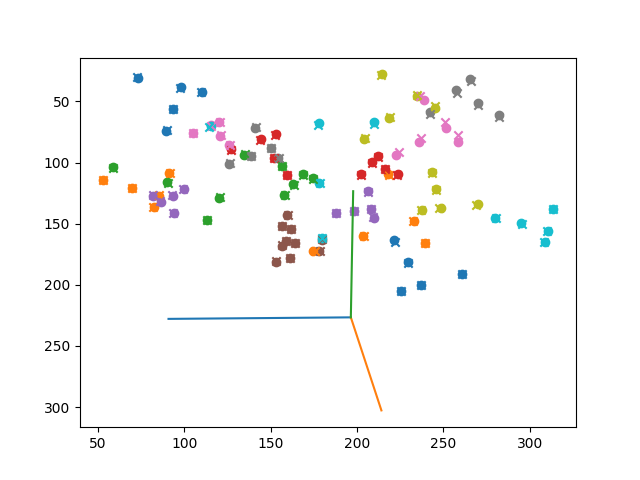
\includegraphics[width=\textwidth]{figure_match.png}
  \caption{\label{figure1} Illustration of the match of measured DV points (crosses) and DV point calculated with the transformation matrix after optimisation (dots).}
\end{figure}

Subsequently, we have used the transformation to project the 3D meshes of tools from the positions and poses detected by the vicon sytem onto the DVS frames with good success.

\subsection{Camera-centric position and pose}
In order to create training data for regressors that predict position and pose of a tool based on DVS data, we need to record position and pose relative to the DVS camera reference frame. Otherwise, the training data, and hence the models, would depend on the (quite likely changing) camera position and orientation.

We were hoping we could use our camera calibration procedure described above to also obtain the transformation from vicon position and pose to DVA-centric position and pose. The idea is that if the camera was essentially like a pinhole camera, then the affine transformation $(A,\vec{n})$ should consist of a rotation  and translation only, i.e. $A \in O(3)$, potentially even $SO(3)$ (depending whether there was an additional flip of an axis or not).
In order to test the idea and design a system for determining camera-centric position and pose, we represented $A$ by Euler angles and repeated our fitting procedure for the set of Euler angles and the translation $\vec{n}$. The resulting fits are slightly less good than in the approach with the general affine transformation (figure \ref{figure2}). Notably, there are some deviations for wand positions very close to the camera. The summed residual error for all points in this example was RMA$= 26.4$ mm.

\begin{figure}
  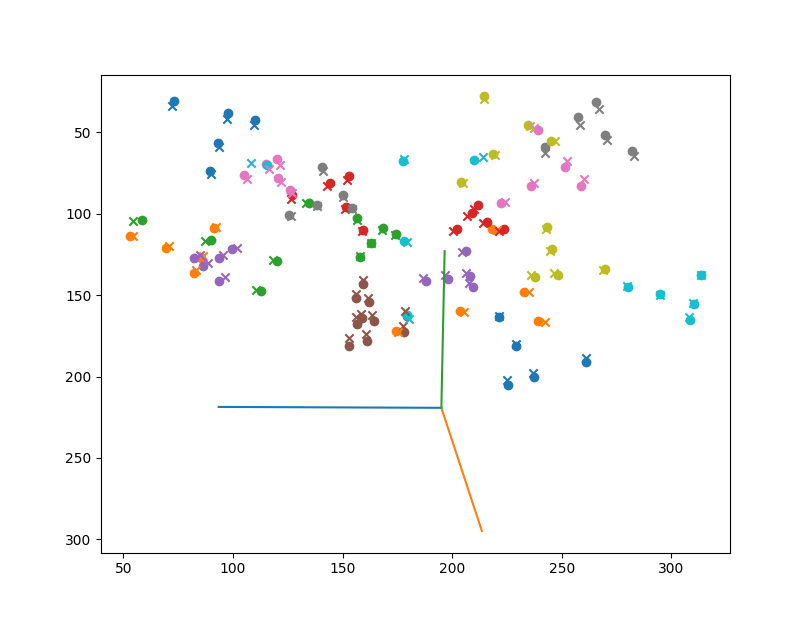
\includegraphics[width=\textwidth]{figure_match_euler.png}
  \caption{\label{figure2} Illustration of the match if fitting with rotation and translation for the affine transformation from vicon to camera centric reference frame. The match is slightly worse than in figure \ref{figure1} with a notable deviation for the very close wand position in cyan.} 
\end{figure}

As the Nelder-Mead algorithm is a simple hill-climbing algorithm, the quality of fits could have been due to being stuck in a local minima. We therefore tried several runs with different parameter combinations using the ``basinhopping'' algorithm. For both approaches, the stated values are the best minimum we were able to find.

It is an interesting question what additional transformation is added to rotation and translation in the ``general affine method''. To analyse this we examined the fitted affine matrix by decomposing it into a rotation matrix and a residual matrix as close as possible to the identity matrix (analyze\_matrix.ipynb). This analysis revealed that the residual transformation that the ``full affine method'' did over the ``rotation+translation method'' was effectively rescaling $z$, whcih is equivalent to rescaling the focal length.

We hence added a rescaling of the focal length to the fitting parameters in addition to the rescaling in $x$ and as a result the fit was essentially as good as with the full affine method.
Figure \ref{figure3} illustrates the result which has error RMS$= 13.56$.

\begin{figure}
  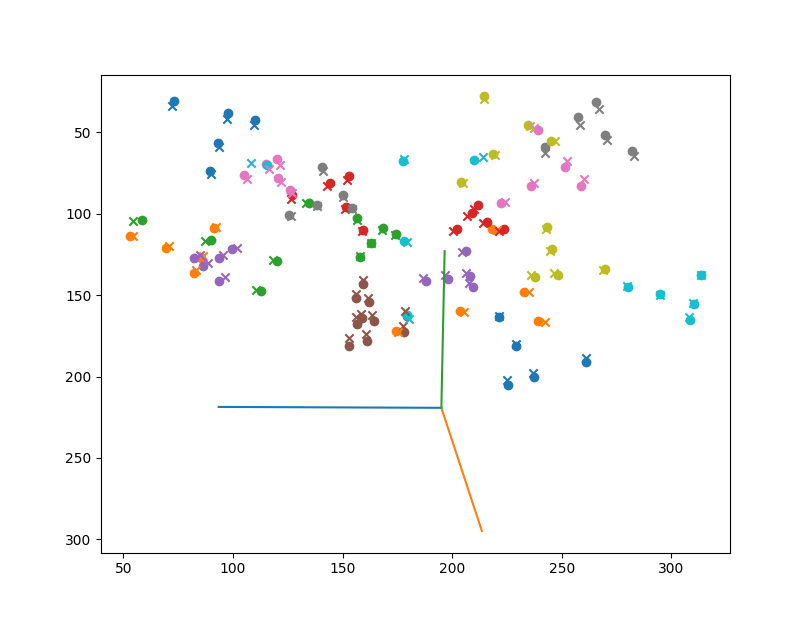
\includegraphics[width=\textwidth]{figure_match_euler.png}
  \caption{\label{figure3} Fitting results after the correction factor fo the focal length was introduced.}
\end{figure}

\subsection{Camera-centric pose estimation}
With these results it appears reasonable to try to use the camera calibration method also in the context of pose estimation relative to camera coordinates. For this purpose one would use the rotation+translation method and then use the determined rotation and translation without the projection stage to transform vicon positions into camera-centric positions. To transform Euler angles for the tool pose, we need to simply combine the Euler angles defining the pose and the Euler angles of the vicon-to-camera rotation.
\end{document}
